\input ../preamble

\begin{document}

{\Huge

  \centerline{\bf TTIC 31230, Fundamentals of Deep Learning}
  \bigskip
  \centerline{David McAllester, Winter 2018}
  \vfill
  \centerline{\bf Deep Graphical Models III}
  \vfill
  \vfill
  \centerline{Expectation Maximization (EM)}
  \vfill
  \centerline{Expected Gradient (EG)}
  \vfill
  \centerline{CTC}
  \vfill
\vfill
\slide{Latent Variable Models}

\begin{eqnarray*}
\Phi^* & = & \argmin_\Phi E_{(x,y) \sim \pop} - \ln Q_\Phi(y|x)
\end{eqnarray*}

\vfill
$y$ ranges over a structured set such as sentences or images.

\vfill
$$Q_\Phi(y|x) = \sum_{\hat{z}} Q_\Phi(\hat{z},y\;|\;x)$$

\vfill
$\hat{z}$ ranges over latent labels such as a word sense for each word or a semantic label for each pixel.

\slide{The Expected Gradient (EG) Identity}

\begin{eqnarray*}
{\color{red} \nabla_\Phi \; \ln Q(y)} & = &  \frac{\nabla_\Phi\; Q(y)}{Q(y)} \\
\\
\\
 & = &  \sum_{\hat{z}}\; \frac{\nabla_\Phi\;Q(\hat{z},y)}{Q(y)} \\
 \\
 \\
  & = &  \sum_{\hat{z}}\; \frac{Q(\hat{z},y)\;  \nabla_\Phi \; \ln Q(\hat{z},y)}{Q(y)} \\
\\
 & = & {\color{red} E_{\hat{z} \sim Q(\hat{z}|y)} \nabla_\Phi \ln Q(\hat{z},y)} \\
\end{eqnarray*}


\slideplain{The EG Identity}


$${\color{red} \nabla_\Phi \; \ln Q_\Phi(y|x) = E_{\hat{z} \sim Q_\Phi(\hat{z}|x,y)} \nabla_\Phi \ln Q_\Phi(\hat{z},y|x)}$$

\vfill
It is important to note that the gradient operation only appears inside the expectation.

\vfill
This is an {\bf expected gradient}.

\slide{Sufficient Statistics}

Consider a model $Q_\Phi(\hat{z},\hat{y}|x)$ and a tensor $S$ computed from $x$, $y$ and $\hat{z}$ such that

\vfill
$${\color{red} E_{\hat{z} \sim Q_\Phi(\hat{z}|x,y)}\;\nabla_\Phi \ln Q_\Phi(\hat{z},y|x) = f\left(E_{\hat{z} \sim Q_\Phi(\hat{z}|x,y)}\;S(x,y,\hat{z})\right)}$$

\vfill
When this equation holds we say that $E_{\hat{z} \sim Q_\Phi(\hat{z}|x,y)}\;S(x,y,\hat{z})$ is a {\bf sufficient statistic} for the model
$Q_\Phi(\hat{z},\hat{y}|x)$.

\vfill
Even when $\hat{z}$ is a structured object (with exponentially many possible values) it is often possible to find a tractable-sized
sufficient statistic that can be computed or estimated efficiently.


\slide{Example: Latent Variable Directed Graphical Models}

\centerline{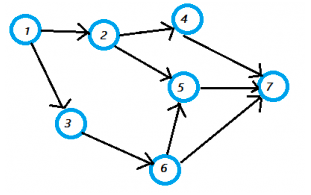
\includegraphics[height=1.5in]{../images/DAG} \hspace{1in} 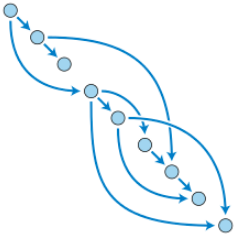
\includegraphics[height=1.5in]{../images/SortedDAG}}

\vfill
We assume a population of pairs $(x,y)$ and a model $Q_\Phi(y|x)$ to be trained by cross-entropy.

\vfill
$$\Phi^* = \argmin_\Phi \;- \ln Q_\Phi(y|x)$$

\vfill
Here $y$ is an assignment values to {\bf observed} nodes.

\vfill
We must marginalize over assignments to {\bf unobserved} nodes.

\slide{Latent Variable Directed Graphical Models}

\centerline{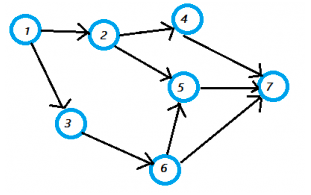
\includegraphics[height=1.5in]{../images/DAG} \hspace{1in} 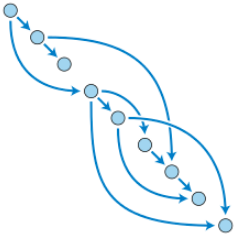
\includegraphics[height=1.5in]{../images/SortedDAG}}

\vfill
Let $\hat{v}$ denote an assignment to all nodes --- both observed and unobserved (latent).

\vfill
Here we consider only directed models --- models satisfying

\vfill
\begin{eqnarray*}
  Q_\Phi(\hat{v}|x) & = & \prod_{i} \; Q_\Phi(x)(\hat{v}[i]\;| \hat{v}[\mathrm{Parents}(i)])
\end{eqnarray*}

\vfill
Here $Q_\Phi(x)$ is a tensor giving the conditional probability tables $Q[\hat{v}[i]\;| \hat{v}[\mathrm{Parents}(i)]]$.

\slide{Observed and Latent Variables}

Let $\hat{v}_y$ be the assignment $\hat{v}$ makes to the observed variables.

\vfill
Let $\hat{v}_z$ be the assignment $\hat{v}$ makes to the unobserved variables.

\vfill
Let $Q$ abbreviate the tensor $Q_\Phi(x)$.
\vfill
$$Q(\hat{v}) = Q(\hat{v}_z,\hat{v}_y)$$

\vfill
$$Q(\hat{v}_y) = \sum_{\hat{v}_z}\;Q(\hat{v}_z,\hat{v}_y)$$

\slide{The Sufficient Statistics}

For each node $i$ the tensor $Q_\Phi(x)$ specifies the conditional probability table $Q[\tilde{v}_i|\tilde{v}_p]$ where $\tilde{v}_i$ ranges over the possible values of node $i$
and $\tilde{v}_p$ ranges over the possible assignments of values to the parents of $i$.

\vfill
$$Q.\grad = \nabla_Q \;- \ln \sum_{\tilde{v}_z} Q(\tilde{v}_z,\tilde{v}_y)$$

\vfill
$$Q.\grad[\tilde{v}_i|\tilde{v}_p] = \frac{- \partial \ln \sum_{\tilde{v}_z} Q(\tilde{v}_z,\tilde{v}_y)}{\partial Q[\tilde{v}_i|\tilde{v}_p]}$$

\slide{The Sufficient Statistics}

\begin{eqnarray*}
\nabla_Q \; \ln \; Q(y) & = & E_{\hat{z} \sim Q(\hat{z}|y)} \nabla_Q \ln Q(\hat{z},y) \\
\\
& = & E_{\hat{z} \sim Q(\hat{z}|y)} \sum_i \nabla_Q \ln Q((\hat{z},y)[i]\;|\; (\hat{z},y)[\mathrm{parents}(i)]) \\
\\
Q.\mathrm{grad}[\tilde{v}_i,\tilde{v}_p]& = & E_{\hat{z} \sim Q(\hat{z}|y)} \frac{1}{Q[\tilde{v}_i,\tilde{v}_p]} \bbone[(\hat{z},y)(i,\mathrm{Parents}(i)) = (\tilde{v}_i,\tilde{v}_p)] \\
\\
& = & \frac{1}{Q[\tilde{v}_i|\tilde{v}_p]} E_{\hat{z} \sim Q(\hat{z}|y)} \bbone[(\hat{z},y)(i,\mathrm{Parents}(i)) = (\tilde{v}_i,\tilde{v}_p)]
\end{eqnarray*}

\vfill
The quantities ${\color{red} E_{\hat{z} \sim Q(\hat{z}|y)} \bbone[(\hat{z},y)(i,\mathrm{Parents}(i)) = (\tilde{v}_i,\tilde{v}_p)]}$ are the {\bf sufficient statistics}.

\slide{Trees are Tractable}

For tree models the sufficient statics can be computed efficiently by message passing (belief propagation).

\vfill
Loopy BP can be used for non-tree models.

\slidetwo{Expected Gradient (EG)}{and Expectation Maximization (EM)}

EG: \hspace{3ex} $\nabla_Q \ln Q(y) = \expectsub{\hat{z} \sim Q(\hat{z}|y)}{\nabla_Q \;\ln Q(\hat{z},y)}$.

\vfill
EM: \hspace{3ex} ${\color{red} Q^{ t+1}} = \argmax_Q \;\expectsub{\hat{z} \sim {\color{red} Q^t}(\hat{z}|y)}{\ln Q(\hat{z},y)}$.

\vfill
EG = $\nabla_Q \ln Q(y)$ equals is the gradient of the EM objective.

\vfill
EG and EM have {\bf the same sufficient statistics} (E-step).

\slidetwo{Connectionist Temporal Classification (CTC)}
{Phonetic Transcription}

A speech signal
$$x = x_1,\; \ldots,\; x_T$$
is labeled with a phone sequence
$$y = y_1, \ldots, y_N$$
with $N << T$ and with $y_n \in {\cal Y}$ for a set of phonemes ${\cal Y}$.

\vfill
The length $N$ of $y$ is not determined by $x$ and the alignment between $x$ and $y$ is not given.

\slide{CTC}
The model defines $Q_\Phi(\hat{z}|x,y)$ where $\hat{z}$ is latent.

\vfill
$$\hat{z} = \hat{z}_1,\;\ldots,\;\hat{z}_T,\;\;\;\hat{z}_t \in {\cal Y} \cup \{\bot\}$$

\vfill
The sequence

\vfill
$$y(\hat{z}) = y_1,\;\ldots,\;y_N$$

\vfill
is the result of removing all the occurrences of $\bot$ from $\hat{z}$.

$$\bot,a_1,\bot,\bot,\bot,a_2,\bot,\bot,a_3,\bot \Rightarrow a_1,a_2,a_3$$

\slide{The CTC Model}

\begin{eqnarray*}
  h_1,\;\ldots,\;h_T & = & \mathrm{RNN}_\Phi(x_1,\;\ldots,\;x_T) \\
  \\
  \\
  Q_\Phi(\hat{z}_t|x_1,\ldots,x_T) & = & \softmax_{\hat{z}} \;e(\hat{z})^\top h_t
\end{eqnarray*}

\vfill
This is a locally normalized (directed) graphical model where $\hat{z}_t$ does not have any parent nodes.

\slide{The Sufficient Statistics}

Since each node has no parents the sufficient statistics are

\vfill
$${\color{red}P_{\hat{z} \sim Q(\hat{z}|y)}(z_t = \tilde{z})}$$

\slideplain{Dynamic Programming (Forward-Backward)}

\begin{eqnarray*}
  x & = & x_1,\;\ldots,\; x_T \\
  \hat{z} & = & \hat{z}_1, \;\ldots,\;\hat{z}_T,\;\;\;\hat{z}_t \in {\cal Y}\cup \{\bot\} \\
  y & = & y_1,\;\ldots,\;y_N,\;\;\;\;y_n \in {\cal Y},\;\;\;N << T \\
  y & = & (\hat{z}_1,\;\ldots,\;\hat{z}_T) - \bot
\end{eqnarray*}
\vfill

Forward-Backward

\begin{eqnarray*}
  \vec{y}_t & = & (\hat{z}_1,\;\ldots,\;\hat{z}_t)-\bot \\
  F[n,t] & = & Q(\vec{y}_t = y_1,\;\ldots,\;y_n) \\
  B[n,t] & = & Q(y_{n+1},\;\ldots,y_N | \vec{y}_t = y_1,\;\ldots,\;y_n)
\end{eqnarray*}

\slide{Dynamic Programming (Forward-Backward)}

\begin{eqnarray*}
  \vec{y}_t & = & (\hat{z}_1,\;\ldots,\;\hat{z}_t)-\bot \\
  F[n,t] & = & Q(\vec{y}_t = y_1,\;\ldots,\;y_n) \\
  B[n,t] & = & Q(y_{n+1},\;\ldots,y_N | \vec{y}_t = y_1,\;\ldots,\;y_n)
\end{eqnarray*}

\begin{eqnarray*}
  F[0,0] & = & 1 \\
  F[n,0] & = & 0 \;\;\;\mbox{for $n > 0$} \\
  F[n+1,t+1] & = & Q(\hat{z}_{t+1} = \bot) F[n+1,t] + Q(\hat{z}_{t+1} = y_{n+1})F[n,t] \\
  \\
  B[N,T] & = & 1 \\
  B[n,T] & = & 0,\;\;\;\mbox{for $n < N$} \\
  B[n-1,t-1] & = & Q(\hat{z}_{t-1} = \bot)B[n-1,t] +  Q(\hat{z}_{t-1} = y_{n-1})B[n,t]
\end{eqnarray*}

\slideplain{Latent Variable MRFs}

\begin{eqnarray*}
  Q_f(\hat{z},\hat{y}) & = & \frac{1}{Z} \; e^{f(\hat{z},\hat{y})}  \\
  \\
  Q_f(\hat{y}) & = & \sum_{\hat{z}}\;Q_f(\hat{z},\hat{y}) \;\; =\;\; \frac{\sum_{\hat{z}} e^{f(\hat{z},\hat{y})}}{Z} \\
  \\
  \\
  Q_f(\hat{y})& = & \frac{Z(\hat{y})}{Z} \\
  \\
  \mathrm{loss}(y) & = & \ln Z - \ln Z(y)
\end{eqnarray*}

\slideplain{The Sufficient Statistics}

\begin{eqnarray*}
  & & {\color{red} P_{\hat{z} \sim Q(\hat{z}|y)}(\hat{z}_t = \tilde{z})} \\
  \\
  \\
  \\
  & = & \frac{1}{Q(y)}\;\sum_n \left\{\begin{array}{ll} F[n,t-1]\;Q(\hat{z}_t)\;B[n,t] & \mbox{for $\hat{z}_t = \bot$} \\
                                            \\
                                            F[n,t-1]\;Q(\hat{z}_t)\;B[n+1,t] & \mbox{for $\hat{z}_t = y_{n+1}$} \\
                                            \\
                                            0 & \mbox{otherwise} \end{array} \right.
\end{eqnarray*}


\slide{Undirected Latent Variable MRFs}
\bigskip
$${\color{red} \Phi^* = \argmin_\Phi \;\;E_{(x,y) \sim \mathrm{Pop}}  -\ln Q_{f_\Phi(x)}(y)}$$
\bigskip
$${\color{red} Q_f(\hat{z},\hat{y})  = \softmax_{\hat{z}, \hat{y}}\;f(\hat{z}, \hat{y})}$$
\bigskip
$${\color{red} f(\hat{z},\hat{y}) = \sum_\alpha  \; f[\alpha,\hat{z}[\alpha],\hat{y}[\alpha]]}$$
\bigskip
$${\color{red} Q_f(\hat{y}) = \sum_{\hat{z}} Q_f(\hat{z},\hat{y})}$$

\slide{Latent Variable MRFs}

\begin{eqnarray*}
  \mathrm{loss}(y,f) & = & \ln Z - \ln Z(y) \\
  \\
  \\
  f.\mathrm{grad}[\alpha,\tilde{y},\tilde{z}]
  & = & {\color{red} P_{\hat{z},\hat{y} \sim Q_f} (\hat{y}[\alpha] = \tilde{y},\hat{z}[\alpha] = \tilde{z})} \\
  \\
  & & - {\color{red} P_{\hat{z} \sim Q_f(\hat{z}|y)} (y[\alpha] = \tilde{y},\hat{z}[\alpha] = \tilde{z})}
\end{eqnarray*}

\vfill
These are the {\bf sufficient statistics} for latent variable MRFs.

\slide{END}

}
\end{document}

